\documentclass{standalone}


\usepackage{tikz}
\usetikzlibrary{shapes,backgrounds,calc,patterns}
\usepackage{venndiagram}


\begin{document}
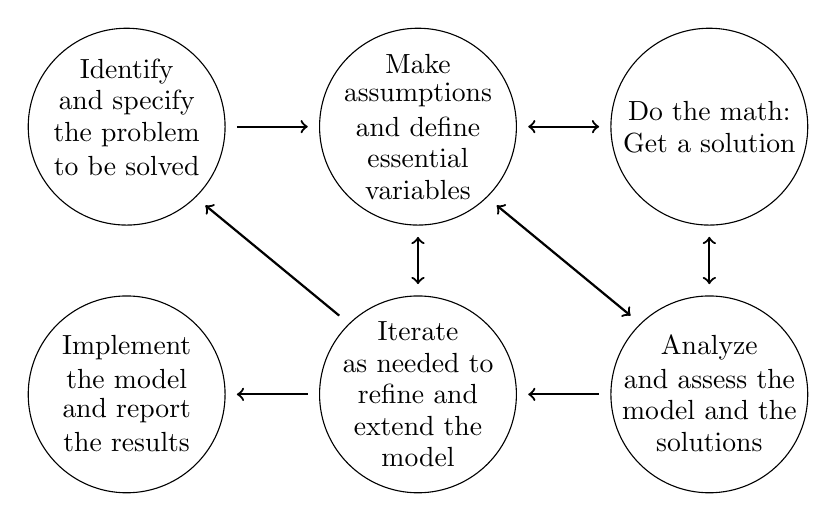
\begin{tikzpicture}
	%    \draw[step=1cm,gray,very thin] (-5,2.5) grid (5,-2.5);
	\draw (-4,1.4) circle (1.25);
	\node at (-4,2.1) {Identify};
	\node at (-4,1.7) {and specify};
	\node at (-4,1.3) {the problem};
	\node at (-4,.9) {to be solved};
	
	\draw (-4,-2) circle (1.25);
	\node at (-4,-1.4) {Implement};
	\node at (-4,-1.8) {the model};
	\node at (-4,-2.2) {and report};
	\node at (-4,-2.6) {the results};
	
	\draw (-.3,1.4) circle (1.25);
	\node at (-.3,2.2) {Make};
	\node at (-.3,1.8) {assumptions};
	\node at (-.3,1.4) {and define};
	\node at (-.3,1) {essential};
	\node at (-.3,.6) {variables};
	
	\draw (-.3,-2) circle (1.25);
	\node at (-.3,(-1.2) {Iterate};
	\node at (-.3,-1.6) {as needed to};
	\node at (-.3,-2) {refine and};
	\node at (-.3,-2.4) {extend the};
	\node at (-.3,-2.8) {model};
	
	
	\draw (3.4,1.4) circle (1.25);
	\node at (3.4,1.6) {Do the math:};
	\node at (3.4,1.2) {Get a solution};
	
	
	\draw (3.4,-2) circle (1.25);
	\node at (3.4,-1.4) {Analyze};
	\node at (3.4,-1.8) {and assess the};
	\node at (3.4,-2.2) {model and the};
	\node at (3.4,-2.6) {solutions};
	
	\draw [->,thick] (-2.6,1.4) -- (-1.7,1.4);
	\draw [<-,thick] (-2.6,-2) -- (-1.7,-2);
	\draw [<->,thick] (1.1,1.4) -- (2,1.4);
	\draw [<-,thick] (1.1,-2) -- (2,-2);
	\draw [<->,thick] (3.4,0) -- (3.4,-.6);
	\draw [<->,thick] (-.3,0) -- (-.3,-.6);
	\draw [->,thick] (-1.3,-1) -- (-3,.4);
	\draw [<->,thick] (2.4,-1) -- (.7,.4);
	
	\end{tikzpicture}
\end{document}